\documentclass[a4paper,AutoFakeBold,AutoFakeSlant]{ctexart}
\usepackage[a4paper,left=2.8cm,right=2.8cm,top=2.5cm,bottom=2.5cm]{geometry}
\usepackage{graphicx}
\usepackage{pythonhighlight}
\usepackage[mathscr]{eucal}
\usepackage{mathrsfs}
\usepackage{booktabs}
\usepackage{capt-of} 
\usepackage{hyperref} 
\usepackage{abstract}
\usepackage{amsmath}
\usepackage{listings}
\usepackage{color}
\usepackage{caption}
\usepackage{subfigure}
\usepackage{enumerate}
\usepackage{amsfonts} 
\usepackage{float}

% -- 中文字体 --
%\setCJKmainfont{Microsoft YaHei}  % 微软雅黑
%\setCJKmainfont{YouYuan}  % 幼圆
%\setCJKmainfont{NSimSun}  % 新宋体
%\setCJKmainfont{KaiTi}    % 楷体
% \setCJKmainfont{SimSun}   % 宋体
%\setCJKmainfont{SimHei}   % 黑体
 
% -- 英文字体 --
\setmainfont{Times New Roman}
% \setmainfont{DejaVu Sans}
% \setmainfont{Latin Modern Mono}
% \setmainfont{Consolas}

\usepackage{xcolor}  	%高亮使用的颜色
\definecolor{commentcolor}{RGB}{85,139,78}
\definecolor{stringcolor}{RGB}{206,145,108}
\definecolor{keywordcolor}{RGB}{34,34,250}
\definecolor{backcolor}{RGB}{220,220,220}

\usepackage{accsupp}	
\newcommand{\emptyaccsupp}[1]{\BeginAccSupp{ActualText={}}#1\EndAccSupp{}}

\usepackage{listings}
\lstset{						%高亮代码设置
	language=python, 					%Python语法高亮
	linewidth=0.95\linewidth,      		%列表list宽度
	%basicstyle=\ttfamily,				%tt无法显示空格
	commentstyle=\color{commentcolor},	%注释颜色
	keywordstyle=\color{keywordcolor},	%关键词颜色
	stringstyle=\color{stringcolor},	%字符串颜色
	%showspaces=true,					%显示空格
	numbers=left,						%行数显示在左侧
	numberstyle=\tiny\emptyaccsupp,		%行数数字格式
	numbersep=5pt,						%数字间隔
	frame=single,						%加框
	framerule=0.1pt,						%划线
	escapeinside=@@,					%逃逸标志
	emptylines=1,						%
	xleftmargin=3em,					%list左边距
	backgroundcolor=\color{backcolor},	%列表背景色
	tabsize=4,							%制表符长度为4个字符
	% gobble=4							%忽略每行代码前4个字符
}




\renewcommand{\abstractname}{}    % clear the title
\renewcommand{\absnamepos}{empty}
%去除摘要两边缩进
\makeatletter
  \renewenvironment{abstract}{%
      \if@twocolumn
        \section*{\abstractname}%
      \else
        \small
        \begin{center}%
          {\bfseries \abstractname\vspace{-.5em}\vspace{\z@}}%
        \end{center}%
      \fi}
      {}
  \makeatother
  \lstset{
    language=Matlab,
    keywords={break,case,catch,continue,else,elseif,end,for,function,
       global,if,otherwise,persistent,return,switch,try,while},
    basicstyle=\ttfamily,
    keywordstyle=\color{blue}\bfseries,
    commentstyle=\color{dkgreen},
    stringstyle=\color{dkpurple},
    backgroundcolor=\color{white},
    tabsize=4,
    showspaces=false,
    showstringspaces=false
 }




\title{\heiti{数学建模HW2实验报告}}
\author{PB19151769~~~~~~马宇骁}

\begin{document}

\maketitle

\begin{abstract}\zihao{-4} \kaishu
\noindent 
\textbf{\heiti 摘要:}从2002年至今,我国经历了5轮猪周期,每轮猪周期持续3-4年。建立数学模型,解释周期性现象,
分析政府和资本在其中的作用,养殖者和消费者的利益如何得到保护。
   \newline
\textbf{\heiti 关键词:}猪周期,政府,资本,消费者,利益
\end{abstract}



\section{背景}


猪周期是一种经济现象,指“价高伤民,价贱伤农”的周期性猪肉价格变化怪圈。“猪周期”的循环轨迹一般是:肉价高——母猪存栏量大增——生猪供应增加——肉价下跌——大量淘汰母猪——生猪供应减少——肉价上涨。

猪肉价格高刺激农民积极性造成供给增加,供给增加造成肉价下跌,肉价下跌到很低打击了农民积极性造成供给短缺,供给短缺又使得肉价上涨,周而复始,这就形成了所谓的“猪周期”。

\section{问题分析}

猪周期是指猪价周期性的波动规律,原理同一般的蛛网模型类似,
本质上是由利润来调节供需变化,并最终反映到价格波动上的一种经济运行方式。
猪周期的前提条件是分散养殖的环境,动力是受利润驱动,核心是周期性的变化,
表现形势是供需错配的循环。“猪周期”的循环轨迹一般遵循:猪价下跌——大量淘汰母猪
——生猪供应减少——猪价上涨——母猪存栏上涨——生猪供应增加——猪价下跌。
市场主体对养殖利润追逐的投机效应,“追涨杀跌,价高伤民,价贱伤农”是对猪周期最通俗
解释。以年为单位,猪周期衡量的是猪价的大周期变化,但是猪价的波动不能仅通过大周期
来解释,在每年内部,同一个周期内部的猪价波动同样频繁,主要受季节性供需的影响,
表现为猪价的季节性规律。把大小两个周期叠加起来观察,会进一步看清猪价在不同周期
内的波动变化细节,还可以进一步将猪价分为“上涨年度”、“触顶年度”、“回落年度”和
“触底年度”。\cite{历次猪周期回顾及本轮周期展望}

具体到细节,可能有以下几种原因:

\begin{itemize}
  \item 生猪生产产量不稳定。生猪生产没有与工业化、城市化同步。一方面中国用地、劳力、资金急剧向工业和城市流动,生猪发展速度减缓;另一方面居民收入快速增加,农村人口大量涌进城市,猪肉需求急剧上升。特别是受比较效益低、疫病难控制及市场风险大等影响,生猪生产产量起伏不定。
  \item 标准化规模饲养程度低。在生猪价格历次波动中,散养户缺乏准确的市场信息和预测能力,只能随生猪价格的涨跌,或盲目扩张生产,或恐慌性退出生产。2011年农业部对全国2000个养猪村的定点监测,养猪户占所有农户的比重为22.74$\%$,仍占不小比例。
  \item 疾病加剧产业波动。如,2006年下半年以来,部分生猪主产省暴发猪蓝耳病疫情,除生猪直接死亡损失外,还导致患病母猪流产或死胎。又如,2010年冬季到2011年春季,一些省区发生仔猪流行性腹泻,个别养殖场小猪死亡率高达50$\%$。疾病导致供应减少,大大推动猪肉价格上涨。
  \item 信息监测预警调控滞后。由于生产分散、单位众多,难以普查,抽检又存在误差等问题,存在着统计数据不准的问题。加之生产者和地方政府出于税收、疫病信息、政策红利等自身利益因素,工作合力不强,没有建立灵敏的监测预警机制,以销定产难度大。
  \item 生猪生长周期性影响。生猪生产具有周期较长、途中难改变的特性。散养户以当年市场价格为标准预期未来收益,陷入“蛛网困境”,生产计划赶不上变化,产量赶不上市场变动的节奏。以2011年猪肉价格上涨为例,既有疫情导致能繁母猪存栏量下降、散养户退出的原因,也有饲料、人工、仔猪等成本迅猛上涨的因素。
\end{itemize}

% \begin{figure}[H]
%   \centering
%   \includegraphics[scale=0.2]{趋势.png}
%   \caption{趋势}
%   \label{}
% \end{figure}

\noindent 
*从本质上看,猪肉价格周期变化的原因可以归结为——\textbf{“供需错配”}。

\begin{itemize}
  \item 生猪养殖周期较长,能繁母猪存栏数量变化到商品猪供给变化历时约10-12个月,产能变化滞后于价格,能繁母猪存栏是生
  猪供给的先行指标。能繁母猪配种后约4个月生产仔猪,再过约6个月商品猪出栏。能繁母猪存栏数量变化大致对应10-12个
  月后生猪供给变化。虽然近年来我国生猪养殖规模化程度有所提高,但出栏量占比仍以散户为主。散户养殖更倾向于直接
  根据猪价决定当期是否养殖,且较难做长期资金规划,故猪价上升,当期增加产能,未来供给增加,猪价下降,当期产能
  下降,未来供给不足的长期规律仍存在。
  \begin{figure}[H]
    \centering
    \includegraphics[scale=0.3]{原因1.png}
    \caption{猪的培育周期}
    \label{}
  \end{figure}
  \item 供需跨期错配形成猪周期波动,供给是周期循环的关键因素。当猪价处于上升周期时,养殖成本相对固定,养殖盈利提升,现
  金流增加。为了增加出栏量获得更多的利润,养殖户补栏种猪或外购仔猪甚至二次育肥,以增加商品猪出栏,增厚利润。当能
  繁母猪存栏增加到一定幅度时,预示着未来10-12个月的商品猪供应增幅较大,可能出现供给过剩,猪价到达峰值回落。当商
  品猪供给开始增加,猪价开始下降,养殖利润减少,供给严重大于需求时,猪价甚至低于育肥成本,养殖亏损,现金流紧张,
  仔猪需求下降。养殖户或者养殖场减少配种,并开始淘汰能繁母猪,能繁母猪存栏下降,产能逐渐去化。当能繁母猪产能下降
  到一定程度时,预示着未来10-12个月商品猪供应减幅较大,可能出现供给不足,猪价触底。
  \begin{figure}[H]
    \centering
    \includegraphics[scale=0.4]{原因2.png}
    \caption{供需错配形成猪周期}
    \label{}
  \end{figure}
\end{itemize}

\begin{table}[H]
\begin{center}
\setlength{\tabcolsep}{5mm}{
  \begin{tabular}{llrrl}
    \toprule 
    猪周期   & 上行周期  & \multicolumn{1}{l}{持续时长(月)} & \multicolumn{1}{l}{增幅} & 外部因素 \\
    \midrule
    2002-2006 & 2002.7-2004.8 & 26    & 70\%  & 非典 \\
    2006-2009 & 2006.8-2008.3 & 20    & 158\% & 猪蓝耳 \\
    2009-2014 & 2009.6-2011.8 & 27    & 111\% &  -\\
    2014-2018 & 2014.5-2016.4 & 24    & 97\%  & 环保政策、猪丹毒 \\
    2018至今 & 2018.6-2021.1 & 32    & 262\% & 非洲猪瘟 \\
\bottomrule
\end{tabular}}
\label{}
\caption{历次猪周期上行期}
\end{center}
\end{table}

\begin{table}[H]
\begin{center}
\setlength{\tabcolsep}{5mm}{
  \begin{tabular}{lllll}
  \toprule 
      猪周期   &下行周期  & 持续时长(月) & 降幅    & 外部因素 \\
    \midrule
    2002-2006 &2004.9-2006.7 & \multicolumn{1}{r}{23} & \multicolumn{1}{r}{-40\%} & 猪链球菌 \\
    2006-2009 &2008.4-2009.5 & \multicolumn{1}{r}{14} & \multicolumn{1}{r}{-49\%} & 猪流感、瘦肉精 \\
    2009-2014 &2011.9-2014.4 & \multicolumn{1}{r}{32} & \multicolumn{1}{r}{-47\%} & 政府收储 \\
    2014-2018 &2016.5-2018.5 & \multicolumn{1}{r}{25} & \multicolumn{1}{r}{-50\%} & - \\
    2018至今 &2021.2至今 & \multicolumn{1}{r}{-}     & \multicolumn{1}{r}{-}      & - \\
    \bottomrule
\end{tabular}}
\label{}
\caption{历次猪周期下行期}
\end{center}
\end{table}

供需是猪周期的决定因素,影响到生猪供给的外因将会带来猪周期的拐点,疫病是历次猪周期最关键的外部因素。生猪疫
病对生猪市场的影响往往具有双向性,一是导致消费者降低消费信心对猪肉的需求减少,二是会使生猪存栏下降。通常情
况下,疫情结束后,猪肉需求量会很快恢复,而生猪生产具有时滞性,难以在短期内补给到位,短期内供需失衡会导致生
猪价格上涨,因此生猪疫病对猪肉市场供给的影响更大,如2006年的猪蓝耳疫病和2018年的非洲猪瘟,都从供给上深刻影
响到猪周期波动。影响需求端的外部因素,如收储制度、食品安全消费受挫,都在短期内影响猪价波动,但难以改变猪周
期变动趋势。





\section{模型建立及分析}

\subsection{模型分析}

\subsubsection{数据收集及初看分析}
为了方便模型建立,选取每年的3,6,9,12月季度性全国生猪平均价格来分析,数据来源于猪易数据\cite{猪易数据}。用Python做趋势图如下图\ref{f3}:

\begin{figure}[H]
  \centering
  \includegraphics[scale=0.65]{trend.png}
  \caption{趋势}
  \label{f3}
\end{figure}


我国生猪价格有着明显的周期变化规律。2000年至今,国内生猪市场经历了4轮比较明显的“猪周期”,分别是2002年6月—2006年5月、
2006年5月—2009年5月、2010年4月—2014年4月、2015年3月—2018年5月,平均每4年生猪价格发生1次周期性的变化,
价格从波谷到波峰上涨幅度分别达$75.52\%, 163.88\%, 100.78\%, 96.61\%$ \cite{2021年我国生猪价格走势及未来市场变化分析}。

\begin{itemize}
  \item 由此,将周期$ T $设置为4年。
\end{itemize}

\subsubsection{数据预处理1:通货膨胀消除}
由于考虑到实际上存在通货膨胀,因此,通过汇聚数据购入中国近20年的CPI数据\cite{CPI},将每年的猪肉价格
除以当年累计CPI的数据(累计以2002年为$t_0$的100)做消除通货膨胀影响之后调整的猪肉价格。

\begin{equation}
  cpi\_ cum_p = 100 \prod \limits_{i=0}^{p} \frac{cpi_i}{100}
\end{equation}

\begin{equation}
  price\_ adj_p = price_p \frac{cpi\_ cum_{\lfloor \frac{p}{4} \rfloor}}{100}
\end{equation}

\begin{figure}[H]
  \centering
  \includegraphics[scale=0.65]{trend1.png}
  \caption{调整趋势}
  \label{f4}
\end{figure}

作图\ref{f4}看到,消除了一个整体明显向上的趋势,但是发现每个波峰波谷都还是有一个上涨的趋势,因此,生猪肉的价格周期在近20年来还是被抬升过的。

% \begin{itemize}
%   \item 由此,如果想继续预测以后年份的生猪价格,只需要将模型进行通货膨胀乘数的加乘处理就能得到真实预测值。
% \end{itemize}

\subsubsection{数据预处理2:HP滤波}
考虑使用HP滤波 (Hodrick Prescott Filter):

Hodrick-Prescott (HP) 过滤器是指数据平滑技术。HP 过滤器通常在分析过程中应用,以消除与商业周期相关的短期波动。
消除这些短期波动揭示了长期趋势。这有助于进行与商业周期相关的经济或其他预测。\cite{Hodrick-Prescott(HP)过滤器是指数据平滑技术}

\begin{itemize}
  \item Hodrick-Prescott 过滤器是指主要用于经济学的数据平滑技术。
  \item 通常在分析过程中用于消除与商业周期相关的短期波动。
\end{itemize}

该方法采用对称的数据移动平均的方法原理,设计滤波器,将变化不定的时间序列数据中具有一定趋势变化的平滑序列分离出来。
于是时间序列数据就被分为两部分:周期性波动数据和趋势要素数据。

设有序列$ Y = \{y_1, y_2, ..., y_r\} $,趋势要素为$ G = \{g_1, g_2,..., g_r\} $,
周期波动要素为$ C = \{c_1,c_2,..., c_r\} $。

记损失函数为$ M $,$ G $被定义为$ M $最小化时的解(即当一系列$ g $的取值使得$ M $的值最小的时候,这个时候的$ G $就是所求的)。

\begin{equation}
  min(M) = min \left\{\sum_{t=1}^{T}(y_t-g_t)^2 + \lambda \sum_{t=3}^{T} \left[(g_t-g_{t-1}) - (g_{t-1}-g_{t-2})\right]^2 \right\}
\end{equation}

其中,$\lambda$为平滑参数,
\begin{equation}
  \begin{aligned}
    M = \ \ &(y_1-g_1)^2 + (y_2-g_2)^2 + \cdots + (y_r-g_r)^2 \\
        & + \lambda \{\left[(g_{3}-g_{2}) - (g_{2}-g_{1})\right]^2 + \left[(g_{4}-g_{3}) - (g_{3}-g_{2})\right]^2 + \cdots\\
        & + \left[(g_{r}-g_{r-1}) - (g_{r-1}-g_{r-2})\right]^2 \} 
  \end{aligned}
\end{equation}

要想$M$取最小值,即要使得后半部分趋于0,即$g_t$和$g_{t-1}$,$g_{t-1}$和$g_{t-2}$之间应该足够接近,即分布在一条直线上。

其中,$ \sum_{t=1}^{T}(y_t-g_t)^2 $刻画了趋势成分$T$对$Y$原序列的跟踪程度;\\
$ \sum_{t=3}^{T} \left[(g_t-g_{t-1}) - (g_{t-1}-g_{t-2})\right]^2 $刻画了趋势$Y$的光滑程度。

\begin{itemize}
  \item 当$\lambda = 0$时,HP滤波退化为最小二乘法,此时当$ y_t = g_t $时,$ M $取得最小值;
  \item $ \lambda $越大,$ T $越平滑;
  \item 当$\lambda \rightarrow \infty$时,估计的趋势将接近线性函数。
\end{itemize}

为求极值,对$M$分别求$g_1, g_2,..., g_T$的一阶导数:
\begin{equation}
  \left\{
  \begin{aligned}
    & \frac{\partial M}{\partial g_1} = 0 \Rightarrow -2(y_1-g_1) + 2\lambda(g_3-2g_2+g_1) = 0\\
    & \frac{\partial M}{\partial g_2} = 0 \Rightarrow -2(y_2-g_2) + 2\lambda(g_4-2g_3+g_2) - 4\lambda(g_3-2g_2+g_1) = 0\\
    & \qquad \ \ \vdots \\
    & \frac{\partial M}{\partial g_T} = 0 \Rightarrow -2(y_T-g_T) + 2\lambda(g_T-2g_{T-1}+g_{T-2}) = 0
  \end{aligned}
  \right.
\end{equation}

最终得到:
\begin{equation}
  \begin{bmatrix}
    I + \lambda
    \begin{pmatrix}
      1	&	-2	&	1	&\cdots&	0	&	0 \\
      -2	&	4+1	&	-2-2&\cdots&	0	&	0 \\
      1	&	-2-2&	1+4+1&\cdots&	0	&	0 \\
      \vdots&\vdots&\vdots&\ddots&\vdots&\vdots \\
      0	&	0	&	0	&\cdots&	1+4	&	-2 \\
      0	&	0	&	0	&\cdots&	-2	&	1
    \end{pmatrix}
  \end{bmatrix}
  \begin{pmatrix}
    g_{1}\\g_{2}\\g_{3}\\ \vdots \\g_{T-1}\\g_{T}
  \end{pmatrix}
  =
  \begin{pmatrix}
    y_{1}\\  y_{2}\\  y_{3}\\ \vdots \\  y_{T-1}\\  y_{T}
  \end{pmatrix}
\end{equation}

记$F$为:
\begin{equation*}
  F = 
  \begin{pmatrix}
    1	&	-2	&	1	&\cdots&	0	&	0 \\
    -2	&	4+1	&	-2-2&\cdots&	0	&	0 \\
    1	&	-2-2&	1+4+1&\cdots&	0	&	0 \\
    \vdots&\vdots&\vdots&\ddots&\vdots&\vdots \\
    0	&	0	&	0	&\cdots&	1+4	&	-2 \\
    0	&	0	&	0	&\cdots&	-2	&	1
  \end{pmatrix}
\end{equation*}

则,$ Y = \left[I + \lambda F\right]G $,$ C = \lambda FG $,$F$中每一列和为0。

由此,当给定$\lambda$时,$Y$已知,则可以解得$G, C$。

于是,根据HP滤波算法,对未消除通货膨胀的20年的生猪价格进行处理,针对不同的$\lambda$值,作图如下图\ref{f5}:

\begin{figure}[H]
  \centering
  \includegraphics[scale=0.5]{hp.pdf}
  \caption{HP滤波结果}
  \label{f5}
\end{figure}

由于根据经济学共识,$\lambda$的取值为年度数据取6.25,季度数据取1600,月度数据取129600。故,选择$\lambda = 1600$的处理为最终的HP滤波处理结果。

接下来检验c序列的正态性:

原假设H0:数据服从正态分布 $N(\mu,\sigma)$ ,其中$\mu$用样本均值代替,$\sigma$用数据的样本修正标准差代替。
将数据从小到大排列,在原假设的条件下计算每一个数据的分布函数P1.
计算每一个数据的累计频率P2进行比较,如果两者之间没有显著性差异,就认为H0成立。

利用Python的scipy.stats库中的kstest进行检验,结果如下:

\begin{itemize}
  \item KstestResult(statistic=0.2144740150301165, pvalue=0.0010408599470181912)
\end{itemize}

证明不可以认为 $95\%$ 的置信水平上c服从正态分布。即波动部分不服从标准正态分布。因此,可以肯定,20年价格的变化不是简单的随机波动,而是有
背后的各类因素的影响形成的。

展示其中的趋势成分g和周期成分c如下图\ref{f6}:
\begin{figure}[H]
  \centering
  \includegraphics[scale=0.7]{gc.pdf}
  \caption{趋势成分g和周期成分c}
  \label{f6}
\end{figure}

可以看出5个周期的趋势。很明显从2018年开始的第五个周期对波动影响很大。根据资料分析:

从 2018 年 8 月我国首次发现非洲猪瘟疫情直到 2019 年的全国蔓延,2019 年国内几乎有三分之一的生
猪死亡,造
成了非常严重的生猪供应缺口,生猪价格从最低 2019 年最低 10 元/公斤上涨至 2019 年 11 月近 40
元/公斤历史高位。随着储备肉投放、进口肉增加,猪价高位回落,但 1 月下旬国内新冠疫情爆发,
各地运输受阻、屠宰企业停工令猪价再度上涨。3 月份国内疫病转好,屠宰企业复工,养殖端加快
生猪出栏、储备肉投放以及进口肉增加,而下游需求受疫病影响超预期下降导致猪价大跌,5 月中
旬生猪价格最低跌至 24 元/公斤,较最高点跌幅达 30。随后养殖端挺价惜售、肥猪供应减少,价
格触底反弹,叠加新发地疫情引发全国冻肉检查,进口肉也减少,助推猪价再度攀升。本轮周期与
以往周期的不同之处在于,价格的上涨并未带来供应的快速恢复,养殖行业的恢复很大程度上仍受
制于非瘟疫情。受到国
家恢复生猪产能的政策鼓励以及超高养殖利润的驱动,2020年3月开始能繁母猪产能快速恢复,对应2021年开始生猪出栏量增加。因此下降速度也明显。

从趋势项可以看出猪肉价格长期是增长趋势。
考虑到上一小节去除通货膨胀的影响,再做去除通货膨胀的HP滤波图(图\ref{f7}):
\begin{figure}[H]
  \centering
  \includegraphics[scale=0.7]{gc_adj.pdf}
  \caption{调整趋势成分g和周期成分c}
  \label{f7}
\end{figure}

发现,确实如上一小节所分析,依然存在价格的长期上涨趋势。


\subsection{ARIMA模型建立}

ARIMA模型全称为自回归移动平均模型(Autoregressive Integrated Moving Average Model,简记ARIMA),是由博克思(Box)和詹金斯(Jenkins)于
70年代初提出的一著名时间序列预测方法,所以又称为box-jenkins模型、博克思-詹金斯法。其中ARIMA(p,d,q)称为差分自回归移动平均模型,AR是自回归, 
p为自回归项; MA为移动平均,q为移动平均项数,d为时间序列成为平稳时所做的差分次数。\ref{ARIMA预测模型}

ARIMA模型的基本思想是:将预测对象随时间推移而形成的数据序列视为一个随机序列,用一定的数学模型来近似描述这个序列。这个模型一旦被识别后就可以从
时间序列的过去值及现在值来预测未来值。现代统计方法、计量经济模型在某种程度上已经能够帮助企业对未来进行预测。

ARIMA(p,d,q)模型可以表示为:

\begin{equation}
  (1 - \sum_{i=1}^{p} \phi_i L_i)(1 - L)^d X_i = (1 + \sum_{i=1}^{q} \theta_i L_i) \varepsilon_i
\end{equation}
其中L是滞后算子(Lag operator),$d \in \mathbb{Z}$.

% ARIMA模型含有三个参数 $p, d, q$:
\begin{itemize}
  \item p--代表预测模型中采用的时序数据本身的滞后数(lags) ,也叫做AR/Auto-Regressive项
  \item d--代表时序数据需要进行几阶差分化,才是稳定的,也叫Integrated项。
  \item q--代表预测模型中采用的预测误差的滞后数(lags),也叫做MA/Moving Average项
\end{itemize}

% 完整表示如下:
% \begin{equation}
%   Y_t = c + \Phi_1 Y_{t-1} + \Phi_2 Y_{t-2} + \cdots + \Phi_p Y_{t-p} + \varepsilon_t + \theta_1\varepsilon_{t-1} + \theta_2\varepsilon_{t-2} + \cdots + + \theta_q\varepsilon_{t-q}
% \end{equation}

ARIMA模型预测的基本程序:
\begin{enumerate}
  \item 根据时间序列的散点图、自相关函数和偏自相关函数图以ADF单位根检验其方差、趋势及其季节性变化规律,对序列的平稳性进行识别。一般来讲,经济运行的时间序列都不是平稳序列。
  \item 对非平稳序列进行平稳化处理。如果数据序列是非平稳的,并存在一定的增长或下降趋势,则需要对数据进行差分处理,如果数据存在异方差,则需对数据进行技术处理,直到处理后的数据的自相关函数值和偏相关函数值无显著地异于零。  
  \item 根据时间序列模型的识别规则,建立相应的模型。若平稳序列的偏相关函数是截尾的,而自相关函数是拖尾的,可断定序列适合AR模型;若平稳序列的偏相关函数是拖尾的,而自相关函数是截尾的,则可断定序列适合MA模型;若平稳序列的偏相关函数和自相关函数均是拖尾的,则序列适合ARMA模型。
  \item 进行参数估计,检验是否具有统计意义。对模型的参数进行估计的方法通常有相关矩估计法、最小二乘估计以及极大似然估计等。
  \item 进行假设检验,诊断残差序列是否为白噪声。 
  \item 利用已通过检验的模型进行预测分析。
\end{enumerate}

\subsubsection{差分阶数d和相关检验}

% d就是差分的阶数,首先通过检验,看原时间序列的平稳性,如果原时间序列是平稳的,那么d=0;
% 如果原数据不平稳,那么做差分,通过检验直到时间序列平稳。一般差分次数不超过2次。

看图\ref{f3},该时间序列是显著不平稳的。因此,做时间序列的acf图来确定阶数。如果acf表现为10阶或以上的拖尾,那么需要进一步的差分,
如果acf表现为1阶截尾,则可能是过度差分了,最好的差分阶数是使acf先拖尾几阶,然后截尾。
\begin{figure}[H]
  \centering
  \includegraphics[scale=0.7]{d.pdf}
  \caption{差分acf}
  \label{f8}
\end{figure}

有的时候,可能在2个阶数之间无法确定用哪个,因为acf的表现差不多,那么就选择标准差小的序列。

上面是原时间序列、一阶差分后、二阶差分后的acf图(图\ref{f8}),可以看到,原序列的acf图的拖尾阶数过高了,而一阶差分后大致是平稳时间序列。
用statsmodels.tsa.stattools库中的adfuller函数进行单位根检验,确定数据为平稳时间序列:
\begin{quotation}
  -4.986603319334445, ADF检验的结果

  2.3588673886572885e-05, P值

  11, 滞后数量

  67, 用于ADF回归和临界值计算的数量

  \{'1\%': -3.5319549603840894,

  '5\%': -2.905755128523123,

  '10\%': -2.5903569458676765\}, 临界值

  324.65299645850484
\end{quotation}
从结果可以看出拒绝原假设,故数据为平稳时间序列。
所以一阶差分更合适。

再Q检验,检验数据是否具有相关性。只有在序列有相关性,即t时刻的y与t-1时刻的y有关系时arma模型才有意义。因此,使用
statsmodels.stats.diagnostic库中的acorr\_ljungbox进行检验,结果如表\ref{t3}:

第一个数:统计值; 第二个数:p值。从结果可以看出,p值较小,拒绝原假设(没有相关性),故数据有序列相关性。
\begin{table}[H]
  \begin{center}
  \setlength{\tabcolsep}{6mm}{
  \begin{tabular}{rrr}
    \toprule
    {} &    lb\_stat &  lb\_pvalue \\
    \midrule
    1  &   2.540868 &   0.110934 \\
    2  &   2.542808 &   0.280438 \\
    3  &   2.632786 &   0.451771 \\
    4  &   3.945452 &   0.413438 \\
    5  &   5.997015 &   0.306510 \\
    6  &  15.313093 &   0.017956 \\
    7  &  23.381720 &   0.001462 \\
    8  &  23.887319 &   0.002394 \\
    9  &  23.987902 &   0.004320 \\
    10 &  24.733571 &   0.005874 \\
    \bottomrule
\end{tabular}
\caption{相关性检验\label{t3}}}
\end{center}
\end{table}



\subsubsection{AR阶数p初定}

AR项表示一个p阶的自回归模型可以表示如下:
\begin{equation}
  y_t = c + \phi_1 y_{t-1} + \phi_2 y_{t-2} + \cdots + \phi_p y_{t-p} + \varepsilon_t
\end{equation}

c是常数项,$\varepsilon_t$ 是随机误差项。
对于一个AR(1)模型而言:
\begin{itemize}
  \item 当 $\phi_1$ = 0 时,yt 相当于白噪声;
  \item 当 $\phi_1$ = 1 并且 c = 0 时,yt 相当于随机游走模型;
  \item 当 $\phi_1$ = 1 并且 c $\neq$ 0 时,yt 相当于带漂移的随机游走模型;
  \item 当 $\phi_1$ < 0 时,yt 倾向于在正负值之间上下浮动。
\end{itemize}

AR的阶数p可以大致通过pacf图来设定,因为AR各项的系数就代表了各项自变量x对因变量y的偏自相关性。

\begin{figure}[H]
  \centering
  \includegraphics[scale=0.51]{p.pdf}
  \caption{差分pacf}
  \label{f9}
\end{figure}

从上图(图\ref{f9})可以看出:5, 6, 7, 18都可以采用,但当阶越大,数据处理难度越高。

\subsubsection{MA阶数q初定}

MA项表示一个q阶的预测误差回归模型可以表示如下:
\begin{equation}
  y_t = c + \varepsilon_t + \theta_1\varepsilon_{t-1} + \theta_2\varepsilon_{t-2} + \cdots + + \theta_q\varepsilon_{t-q}
\end{equation}

c是常数项,$\varepsilon_t$是随机误差项。yt 可以看成是历史预测误差的加权移动平均值,q指定了历史预测误差的期数。

MA阶数可以粗略通过acf图来设定,因为MA是预测误差,预测误差是自回归预测和真实值之间的偏差。

\begin{figure}[H]
  \centering
  \includegraphics[scale=0.51]{q.pdf}
  \caption{差分acf}
  \label{f10}
\end{figure}
从上图(图\ref{f10})可以看出:这里可以选择6, 7。

\subsubsection{信息准则定阶}

AIC(Akaike Information Criterion):
\begin{equation}
  AIC = -2 log(L) + 2(p + q + k + 1)
\end{equation}
L是数据的似然函数,k=1表示模型考虑常数c,k=0表示不考虑。最后一个1表示算上误差项,所以其实第二项就是2乘以参数个数。

AICc(修正过的AIC):
\begin{equation}
  AICc = AIC + \frac{2(p+q+k+1)(p+q+k+2)}{T-p-q-k-2}
\end{equation}

BIC(Bayesian Information Criterion):
\begin{equation}
  BIC = AIC + \left[log(T)-2\right](p+q+k+1)
\end{equation}

注意事项: 
\begin{itemize}
  \item 信息准则越小,说明参数的选择越好,一般使用AICc或者BIC。
  \item 信息准则的好处是可以在用模型给出预测之前,就对模型的超参做一个量化评估,这对批量预测的场景尤其有用,因为批量预测往往需要在程序执行过程中自动定阶。
\end{itemize}

因此,继续利用statsmodels.tsa.stattools库arma\_order\_select\_ic硬解,选择AICc作为定阶的参数,结果返回如下:
\begin{quotation}
  (5, 3)
\end{quotation}
即,选择p = 5,q = 3的模型参数: ARIMA(5, 1, 3).


\subsubsection{构建ARIMA模型}

ARIMA(5, 1, 3)的summary如下:
\begin{figure}[H]
  \centering
  \includegraphics[scale=0.85]{output.pdf}
  % \caption{ARIMA模型}
  % \label{ARIMA模型}
\end{figure}

看出,$P>|z|$ 都很小,证明模型拟合良好。

不妨令 $Y_t = y_t - y_{t-1}$ ,则:
\begin{equation}
  \begin{aligned}
    \hat{Y_t} =  &\ \ 1.4157 Y_{t-1} - 1.953 Y_{t-2} + 0.6124Y_{t-3} + 0.1140Y_{t-4} - 0.3766 Y_{t-5}  \\
                &+ \varepsilon_t - 1.4221\varepsilon_{t-1} + 1.2043\varepsilon_{t-2} - 0.5999\varepsilon_{t-3}
  \end{aligned}
\end{equation}

\subsubsection{残差检验}

\begin{figure}[H]
  \centering
  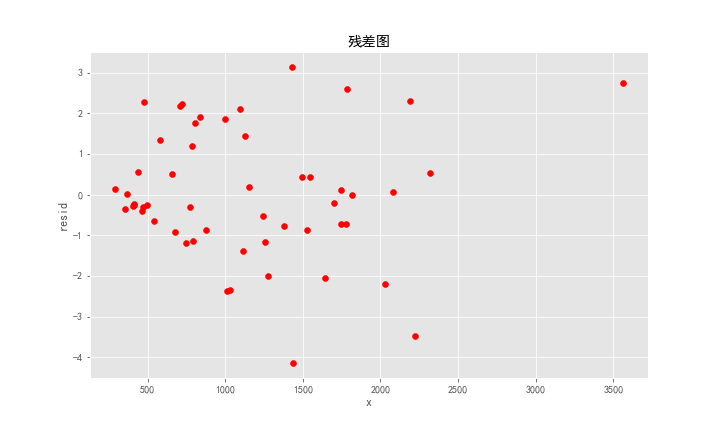
\includegraphics[scale=0.4]{res.pdf}
  \caption{模型残差}
  \label{f11}
\end{figure}
通过scipy库的normaltest对残差进行正态性检验,结果如下:
\begin{quotation}
  NormaltestResult(statistic=8.880217789978431, pvalue=0.01179465407108995)
\end{quotation}
p < 0.05,接受备择假设,认为残差具有正态性,随机误差分布(均值为0的正态分布),说明模型拟合的良好。

如果残差是白噪声序列,说明时间序列中有用的信息已经被提取完毕了,剩下的全是随机扰动,是无法预测和使用的。

残差序列如果通过了白噪声检验,则建模就可以终止了,因为没有信息可以继续提取。

如果残差如果未通过白噪声检验,说明残差中还有有用的信息,需要修改模型或者进一步提取。
\begin{figure}[H]
  \centering
  \includegraphics[scale=0.45]{qq.pdf}
  \caption{qq散点}
  \label{f12}
\end{figure}
图\ref{f12}展示qq散点\footnote{QQ plot的全称是Quantile-Quantile Plot,即分位数-分位数图。如果两个分布相似,则该Q-Q图趋近于落在y=x线上。如果两分布线性相关,则点在Q-Q图上趋近于落在一条直线上,但不一定在y=x线上。Q-Q图可以用来可在分布的位置-尺度范畴上可视化的评估参数。}
基本在直线上。因此可以认为是高斯白噪声,通过白噪声检验,建模可以终止。

\subsubsection{原数据和预测数据对比}

\begin{figure}[H]
  \centering
  \includegraphics[scale=0.475]{forecast.pdf}
  \caption{原数据和预测数据对比}
  \label{f13}
\end{figure}
通过观察预测值与实际值折线图,可以直观看出该模型拟合程度良好。

\subsubsection{未来预测}

利用建立好的ARIMA模型,向后预测5个季度的猪肉价格,并和已经产生的2022年第一季度的数据对照(见表\ref{t4}):
可以看出,对于已经过去的2022第一季度的价格预测非常准确!     
\begin{table}[H]
  \begin{center}
  \setlength{\tabcolsep}{6mm}{
  \begin{tabular}{lrr}
    \toprule
    年月 &    预测值/元 &  真实值/元 \\
    \midrule
    2022-3  &   13.361578 &   13.68 \\
    2022-6  &   13.759277 &   - \\
    2022-9  &   19.540019 &   - \\
    2022-12  &  24.227725  &   - \\
    2023-3  &   24.137864 &   - \\
    \bottomrule
\end{tabular}
\caption{未来预测\label{t4}}}
\end{center}
\end{table}                                            

\begin{figure}[H]
  \centering
  \includegraphics[scale=0.55]{predict.pdf}
  \caption{未来10个季度预测及预测区间}
  \label{f14}
\end{figure}

再展示向后十个季度的预测及95\%置信区间(图\ref{f14})。
可以预测,2022年第一二季度将是第五个猪周期的结束的时间段,也是下一个猪周期的开始,且预估在2024第一季度达到第六轮猪周期的价格顶点27.901545元,然后价格开始再次下跌。


\subsection{小结}

实证中得到如下结论:运用HP滤波技术分
析,我国生猪价格长期是增长趋势,短期内由于政治
经济环境等因素处于波动状态;根据3.2.6的分
析,可知建立的ARIMA(5,1,3)模型精确性较高,
能够较好拟合我国生猪价格变化规律,可为未来消费者消费和养殖户饲养猪计划提供参考。

当运用模型去解释现实中某类经济现象时,
一般不可能将所有影响因素都考虑到模型中。
ARIMA模型的优势在于可以将序列看成一个黑
匣子,然后不考虑序列是如何构成的,但可以利用
数据自身性质去拟合。非平稳数据建立经典回归
模型会出现虚假回归,因此对于我国生猪价格序列,
建立ARIMA模型比传统因果关系模型更为适
合。对于预测其他各省市地区的生猪价格时,可以采
用本文类似的方法,建立时序模型去拟合和评价。\cite{基于HP滤波和ARIMA模型的我国GDP分析与预测}



\section{总结与建议}

\subsection{5轮周期回顾}

第一轮猪周期——“非典”+“惠农政策”共同作用。
该轮周期导致猪价波动的因素主要有:(1)“非典”疫情减少消费,拉低猪价;(2)惠农政
策提振猪价。“非典”疫情从两个方面影响猪价:一是疫情使社会餐饮零售总额显著下降,对猪类
产品需求减少,价格快速下跌;二是疫情隔离措施致使流通环节受阻,产区出栏猪不能外运,非产
区需求得不到满足,对局部市场造成冲击,供求结构失衡。2003 年到 2006 年,政府提高对“三农
“的重视,实行补贴、税收减免、最低收购价等一系列惠农政策,致使农民人均收入增加,购买力
增强,带动猪肉消费需求增加,促使猪价在疫情缓解后快速回暖 。

第二轮猪周期——猪价为疫情左右。2006 年
初猪肉价格持续处于 6.7 元/公斤低位,致使养猪业处于亏损状态,大量母猪被淘汰。而且夏季猪蓝
耳病疫情开始大规模爆发,2006 年全国能繁母猪和生猪存栏量同比降幅 3%左右,生猪供应严重不足,
猪价持续快速上涨。随着 2007 年 8 月蓝耳病疫情开始得到缓解,猪价出现一定幅度回落,但供应不
足使得猪价在短暂回调后立即出现反弹,2008 年 3 月份猪价达到此轮周期的高点 17.5 元/公斤。之
后,受能繁母猪存栏量不断增加,猪肉价格开始进入下行通道,叠加 2009 年甲型 H1N1(猪流感)
疫情爆发,以及出现瘦肉精和注水猪肉等食品安全事件,公众的消费信心受挫,需求阶段性下降,
对猪肉价格形成进一步压制。直到 2009 年 6 月,为防止猪价过度下跌,政府启动冻肉储备,一次性
收储 11.5 万吨,令猪价反弹,但 2009 年产能过剩,猪价从 2010 年初滞涨回落至 9.6 元/公斤。

第三轮猪周期——受猪周期内生动力推动。
本轮周期外部干扰因素较少,主要受猪周期内生动力推动,上一轮周期价格下跌导致养殖户大量淘汰母猪,叠加 2010
年 4—6 月国家及地方政府多次启动冻肉储备项目,生猪供不应求导致猪价从 10 元/公斤低位持续上
涨。随着盈利改善后存栏量持续上升,2011 年中期生猪供求局面反转,猪价出现小幅回落,不过四
季度旺季猪肉需求上升,猪价出现再度上涨,2011 年 9 月份猪价达到此轮周期的高点 19.9 元/公斤。
随着能繁母猪存栏和生猪存栏的持续增加,2012 年母猪存栏和生猪存栏达到历年高位,猪价进入下
行通道。不过夏季过后到年底需求旺季,猪价略有反弹。随着猪肉价格的高涨,养殖户纷纷增加后
备母猪存量,猪肉价格又一次进入下行通道,虽然 2013 年 5 月,为了稳定猪肉价格,商务部等三部
委联合开启冻猪肉收储工作,提振了市场信心,短期价格有所恢复,但随着反腐工作深入和打击“三
公消费”,2014 年猪肉价格再次下行至 10.5 元/公斤。

第四轮猪周期——猪价受环保政策影响。
这一轮周期主要源于环保
政策的严格化,规模化转型调整拉长了周期跨度。生猪养殖业对水资源的需求量高、污染大,与环
境保护的矛盾日益突出,自 2014 年起,我国开始实施严格的环保禁养规定,着力提升生猪养殖业的
规模化程度,导致大量散养户退出市场,生猪和能繁母猪存栏进入持续下降通道,叠加 2015 年上半
年爆发猪丹毒疫情,猪价从 10.5 元/公斤涨至 2016 年 6 月最高 21.2 元/公斤。此轮猪周期的特点是
受环保和规模化影响,猪肉价格上行并未带动生猪显著补栏,可以看到能繁母猪和生猪存栏从 2015
年后均下滑,不过规模化养殖提升了产业效率,一方面提升了生猪的单体重量,另一方面 MSY 提高,
能繁母猪提供的仔猪数量上升,2017 年生猪出栏量不降反增,猪价在 2016 年攀顶之后开始进入下
滑通道,2018 年年后生猪行业亏损不断扩大,并在 2018 年中完成筑底,猪价最低达到 10 元/公斤。

本轮超级猪周期期——非洲猪瘟驱动新一轮超级猪周期。
从存栏看本轮上行周期,期初低水平能繁母猪存栏为大级别猪周期埋下伏笔,突发非洲猪瘟让母猪产能雪上加霜,国内新冠疫情可控后需求恢复
激化供需矛盾。从存栏看本轮下行周期,前期超高利润推动能繁母猪产能快速恢复,全球饲料原料高价推高养殖成本加深亏损,母猪产能去化刚刚开始。

\subsection{建议}
生猪价格周期性波动给生产者造成巨大经济损失, 影响其供求平衡与市场稳定, 是长期困扰生
猪生产发展、价格稳定以及市场供应的难题。而且猪肉价格的大起大落涉及民生问题,学会应对猪周
期,减弱其对宏观经济和人民生活的影响至关重要。
\begin{enumerate}
  \item 加快发展规模化养殖:从 2006 年开始, 生猪行业大量散养户每年以 1\%的速度退出, 生猪规模化的比例不断上
  升, 但散养户仍然占有很大的比重。散养户的组织化程度较低, 造成中国生猪生产、加工与销售的
  脱节, 抵御经营风险的能力始终是比较弱的, 而且供需失衡还会导致游资的介入, 从而加剧市场的
  波动。通过各种扶持、鼓励措施, 发展生猪的规模化生产, 增强养猪业应对市场风险的能力, 这是
  加快跳出生猪周期性大幅波动的关键。 2、建立完善的猪价预警信息系统
  \item 建立完善的猪价预警信息系统:2、建立完善的猪价预警信息系统 
  此外国家要进一步完善信息服务,提供完整、准确、及时的信息, 避免信息不对称造成的失误, 
  还要及时发布市场、技术、疫病信息,保障这些信息获取方式的方便快捷。
  \item 完善生猪保险政策:我国目前开展的生猪保险仅有能繁猪保险、育
  肥猪保险和生猪价格指数保险 3 种常见保险险种。可以提高能繁母猪、育肥猪保险保额,立足于长
  期稳定生猪生产,鼓励具备条件的地方把握时间窗口,持续开展并扩大生猪价格保险试点。
  \item 加快推出生猪期货:生猪现货市场对供求的引导具有滞后性, 使生猪价格周期性波动成为其难以克服的缺陷。期货具有
  发现价格、规避风险的功能,生猪期货也不例外。生猪养殖者通过期货交易行情,及时了解未来的生
  猪市场价格走势,合理调整养殖规模和饲养周期, 从而降低生产经营的盲目性,使得市场上的生猪得
  到长期稳定的供应。
  \item 生猪产业要不断提高技术和管理水平:通过技术和装备的提升, 带动标准化养殖技术的深入推进, 从而实现品种良种化、生产设施
  化、养殖标准化、产品安全化、防疫制度化, 加快传统养猪向现代养猪的新跨越。\cite{4月证监会近日批}
\end{enumerate}



% 接下来验证c序列的平稳性:

% 设{$X_t$}是一时间序列,对任意正整数m,任取t1、t2、t3、...、tm $\in$ T,对任意整数$\tau$,如果{$X_t$}满足以下三个条件:
% \begin{enumerate}
%   \item 任取t $\in$ T,有E($X_t$·$X_t$) $<\infty$;
%   \item 任取t $\in$ T,有E ($X_t$) = $ \mu $ 为常数;
%   \item 任取t,s,k $ \in $ T,且k+s-t $ \in $ T,有$ \gamma $ (t, s) = $ \gamma $ (k, k+s-t)
% \end{enumerate}
% 则称{$X_t$}为宽平稳时间序列。





\section*{代码附录}
部分\textsc{Python}程序代码显示如下:
\begin{python}
  import pandas as pd
  import numpy as np
  import matplotlib as mpl
  import matplotlib.pyplot as plt
  import statsmodels.api as sm
  from scipy.stats import kstest
  from statsmodels.graphics.tsaplots import plot_acf, plot_pacf

  data0 = pd.read_excel(r'数据.xls')
  data = pd.read_excel(r'data.xls')
  name = data.columns

  # 设置绘图风格
  plt. style.use("ggplot")
  # 设置中文编码和符号的正常显示
  plt.rcParams["font.sans-serif"] = "SimHei"
  plt.rcParams["axes.unicode_minus"] = False
  # 设置图框的大小
  fig = plt.figure(figsize = (10,6))
  # 绘图
  plt.ylim(0, 40)
  plt.plot(data.loc[:,name[0]], # x轴数据
          data.loc[:,name[1]], # y轴数据
          linestyle = '-', # 折线类型
          linewidth = 2, # 折线宽度
          color = 'steelblue', # 折线颜色
          marker = 'o', # 点的形状
          markersize = 4, # 点的大小
          markeredgecolor='black', # 点的边框色
          markerfacecolor='brown') # 点的填充色
  # 添加标题和坐标轴标签
  plt.title('7月全国生猪平均价格-年份趋势图')
  plt.xlabel('年份')
  plt.ylabel('7月全国生猪平均价格/元')
  plt.savefig('trend.png')
  # 显示图形
  plt.show()
\end{python}

\begin{python}
  cpi_cum = [100]
  cpi = data0['cpi']
  for i in range(1,20):
      c = cpi_cum[i-1]*cpi[i]/100
      cpi_cum.append(c)
  data0['cpi_cum'] = cpi_cum
  price_adj = []
  price = data['猪肉价格']
  for i in range(len(price)):
      c = i // 4
      p = price[i]*100/cpi_cum[c]
      price_adj.append(p)
  data['调整猪肉价格'] = price_adj
\end{python}

\begin{python}
  datap = data[[name[0],name[2]]]
  def hp(y, lamb=10):
    def D_matrix(N):
        #(N-1,N) 元素全为0
        D = np.zeros((N-1,N))
        #后(N-1,N-1)对角线元素置1
        D[:,1:] = np.eye(N-1)
        #前(N-1,N-1)对角线元素置-1
        D[:,:-1] -= np.eye(N-1)
        return D

    N = len(ts)
    D1 = D_matrix(N)
    D2 = D_matrix(N-1)
    D = D2.dot(D1) 
    g = np.linalg.inv((np.eye(N)+lamb*D.T.dot(D)).dot(ts)
    c = lamb*D.T.dot(D).dot(g)
    return g,c

  N = len(datap)
  ts = price
  plt.figure(figsize=(15,15))

  # 尝试不同的lamda
  for i,l in enumerate([0.1,1,10,100,1000, 10000]):
      plt.subplot(3,2,i+1)
      g,c = hp(ts,l)
      plt.plot(ts, label='original')
      plt.plot(g, label='filtered')
      plt.legend()
      plt.title('$\lambda$='+str(l))
  plt.show()

  g,c = hp(price_adj,10)
  data['hp_g'] = g
  data['hp_c'] = c
\end{python}

\begin{python}
  plt.rcParams.update({'figure.figsize':(9,7), 'figure.dpi':120})

  df = data[name[1]]

  # Original Series
  fig, axes = plt.subplots(3, 2, sharex=True)
  axes[0, 0].plot(df); axes[0, 0].set_title('Original Series')
  plot_acf(df, ax=axes[0, 1])

  # 1st Differencing
  axes[1, 0].plot(df.diff()); axes[1, 0].set_title('1st Order Differencing')
  plot_acf(df.diff().dropna(), ax=axes[1, 1])

  # 2nd Differencing
  axes[2, 0].plot(df.diff().diff()); axes[2, 0].set_title('2nd Order Differencing')
  plot_acf(df.diff().diff().dropna(), ax=axes[2, 1])

  # plt.savefig('d.pdf')
  plt.show()

  data_diff = df.diff()
  data_diff = data_diff.dropna()
  from statsmodels.tsa.stattools import adfuller
  adfuller(data_diff)

  from statsmodels.stats.diagnostic import acorr_ljungbox
  acor = acorr_ljungbox(data_diff, lags = 10)
  print(acor.to_latex(index=True))
\end{python}

\begin{python}
  import statsmodels.tsa.stattools as st

  model = st.arma_order_select_ic(data_diff, max_ar=8, max_ma=8, ic=['aicc', 'bic', 'hqic'])
  model.aicc_min_order #返回一个元组,分别为p值和q值
\end{python}

\begin{python}
  from statsmodels.tsa.arima.model import ARIMA

  df.rename('price',inplace=True)
  model = ARIMA(df, order=(5,1,3))
  result = model.fit()
  result.summary()
  plt.rc('figure', figsize=(12, 7))
  #plt.text(0.01, 0.05, str(model.summary()), {'fontsize': 12}) old approach
  plt.text(0.01, 0.05, str(result.summary()), {'fontsize': 10}, fontproperties = 'monospace') # approach improved by OP -> monospace!
  plt.axis('off')
  plt.tight_layout()
  # plt.savefig('output.pdf')
  plt.rcParams.update({'figure.figsize':(18,6), 'figure.dpi':200})
  residuals = pd.DataFrame(result.resid)
  fig, ax = plt.subplots(1,2)
  residuals.plot(title="Residuals", ax=ax[0])
  residuals.plot(kind='kde', title='Density', ax=ax[1])
  # plt.savefig('res.pdf')
  plt.show()
  resid = result.resid
  plt.rcParams.update({'figure.figsize':(12,7), 'figure.dpi':200})
  from statsmodels.graphics.api import qqplot

  qqplot(resid, line='q', fit=True)
  # plt.savefig('qq.pdf')
  plt.show()

  yhat = result.predict(start=1, end =len(data) )
  plt.rcParams.update({'figure.figsize':(10,6), 'figure.dpi':100})
  plt.plot(data.loc[:,'年月'],df, label='data')
  plt.plot(data.loc[:,'年月'],yhat, label='forecast')
  plt.legend()
  # plt.savefig('forecast.pdf')
plt.show()
\end{python}

\begin{python}
  # Create Training and Test
  train = date[:80]#['猪肉价格']
  test = date[79:]

  # Forecast
  fc= result.predict(start=len(data), end =len(data) + 10 )  # 95% conf
  pred_dynamic = result.get_prediction(start=len(data),end =len(data) + 10,  dynamic=True, full_results=True, alpha=0.05)
  pred_dynamic_ci = pred_dynamic.conf_int()

  # Make as pandas series
  fc_series = pd.Series(list(fc), index=list(date[79:]['年月']))
  lower_series = pd.Series(pred_dynamic_ci.values[:, 0], index=list(date[79:]['年月']))
  upper_series = pd.Series(pred_dynamic_ci.values[:, 1], index=list(date[79:]['年月']))

  # Plot
  plt.figure(figsize=(12,5), dpi=100)
  plt.plot(train.loc[:,'年月'],train.loc[:,'猪肉价格'], label='training')
  # plt.plot(test, label='actual')
  plt.plot(fc_series, label='forecast')
  plt.fill_between(lower_series.index, lower_series, upper_series, 
                  color='k', alpha=.15)
  plt.title('Forecast vs Actuals')
  plt.legend(loc='upper left', fontsize=8)
  # plt.savefig('predict.pdf')
  plt.show()
\end{python}

\bibliographystyle{ieeetr}
\bibliography{bibl}

\end{document}
